    \begin{frame}{Cảm hứng từ sinh học}
        \begin{columns}
        \column{0.5\textwidth}
		\begin{itemize}
    		\begin{block}{Nền tảng}
    		    \begin{itemize}
    		    \item Được gọi là các mạng Nơ-ron nhân tạo, mô phỏng tổ chức thần kinh tự nhiên.
    		    \item Các nơ-ron đơn lẻ được gọi là các perceptron
    		    \item Thực chất là các mô hình toán học đơn giản định nghĩa một hàm $f: X \rightarrow Y$
    		    \end{itemize}
    		\end{block}
    		\begin{block}{Ứng dụng}
    		    \begin{itemize}
    		    \item Là cốt lõi của các mô hình Học sâu như CNN, RNN vv...
    		    \item Các bài toán hệ thống tự nhận diện, điều khiển, khai phá dữ liệu vv...
    		    \end{itemize}
    		\end{block}
		\end{itemize}
		\column{0.48\textwidth}
		\begin{figure}[ht]
            \centering
            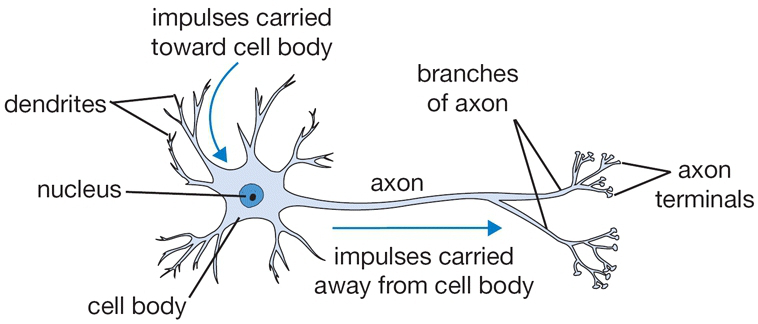
\includegraphics[width=1.0\linewidth]{images/neuron-net.png}
            \caption{Nơ-ron sinh học}
            \label{fig:problem:neural-architect}
            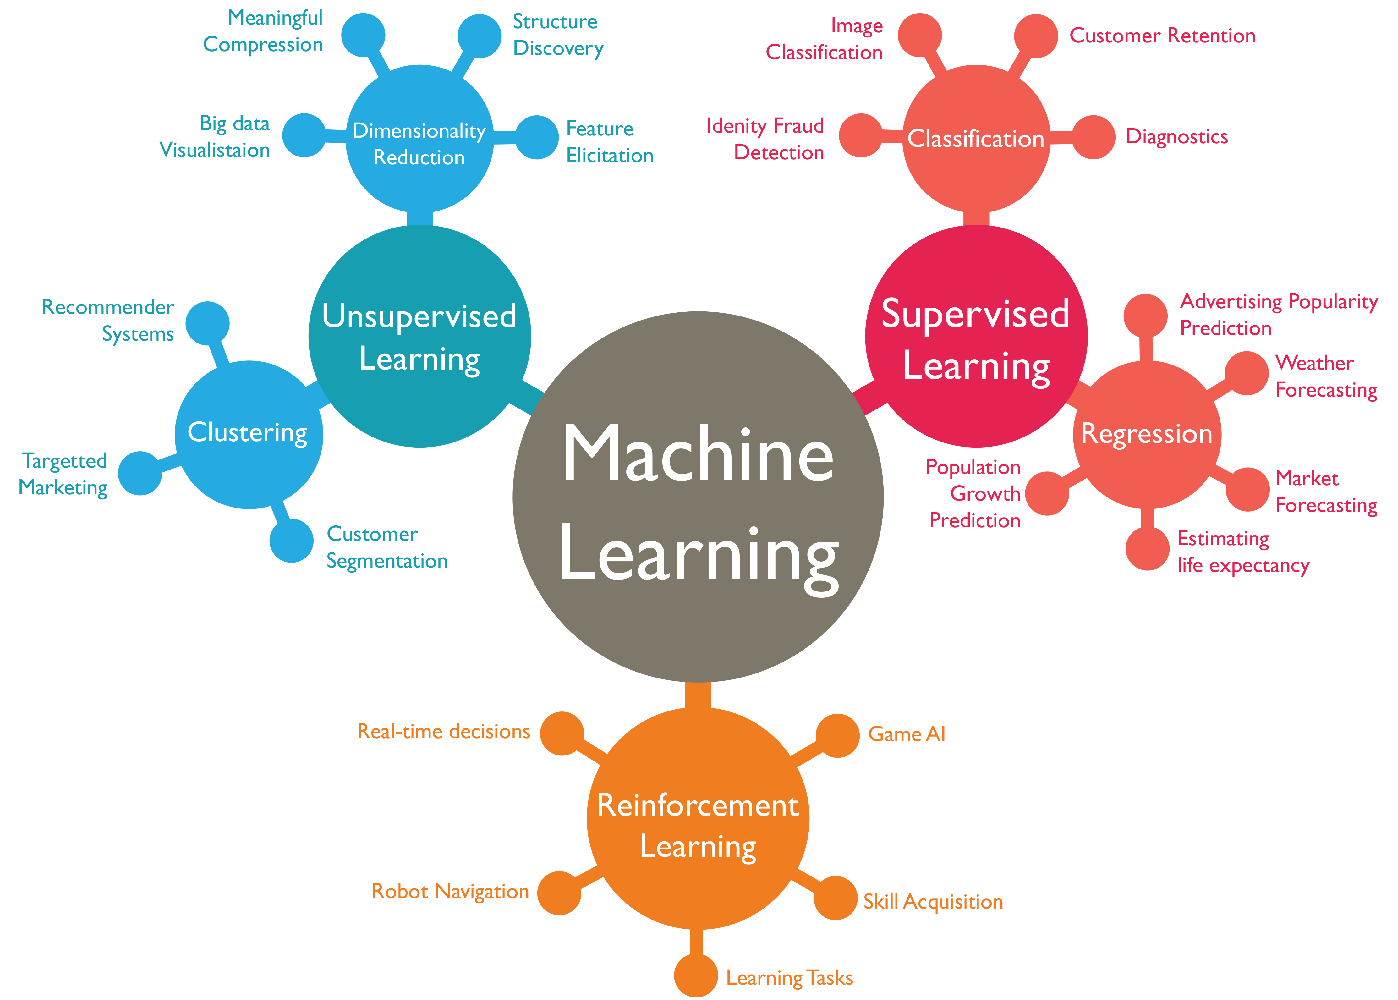
\includegraphics[width=1.0\linewidth, height=3cm]{images/machine.png}
            \caption{Học máy}
        \end{figure}
        
		\end{columns}
	\end{frame}
	
	\begin{frame}{Kiến trúc mạng Nơ-ron}
        \begin{columns}
        \column{0.45\textwidth}
		\begin{itemize}
    		\begin{block}{Kiến trúc mạng Nơ-ron}
    		     \emph{Perceptron} đa tầng: \emph{Lớp Input, Lớp Hidden, Lớp Output}.
    		\end{block}
    		\begin{block}{Mạng Nơ-ron lan truyền tiến}
    		    Mỗi nốt ở tầng nào đó sẽ nhận đầu vào từ các nốt ở tầng trước đó mà không có chiều suy luận ngược lại:
    		    \begin{equation}
                  \begin{array}{l}
                    z_i^{l+1} = \sum_{j=1}^{n^{(l)}}w_{ij}^{(l+1)}a_j^{(l)} + b_j^{(l+1)} \\
                    \\
                    a_i^{(l+1)} = g(z_i^{(l+1)})
                  \end{array}
                \end{equation}
                \textbf{Hàm chi phí:} $C: F \rightarrow R$ sao cho lời giải tối ưu $f^*, C(f^*)  \leq C(f) \forall f \in F$
    		\end{block}
		\end{itemize}
		\column{0.53\textwidth}
		\begin{figure}[ht]
            \centering
            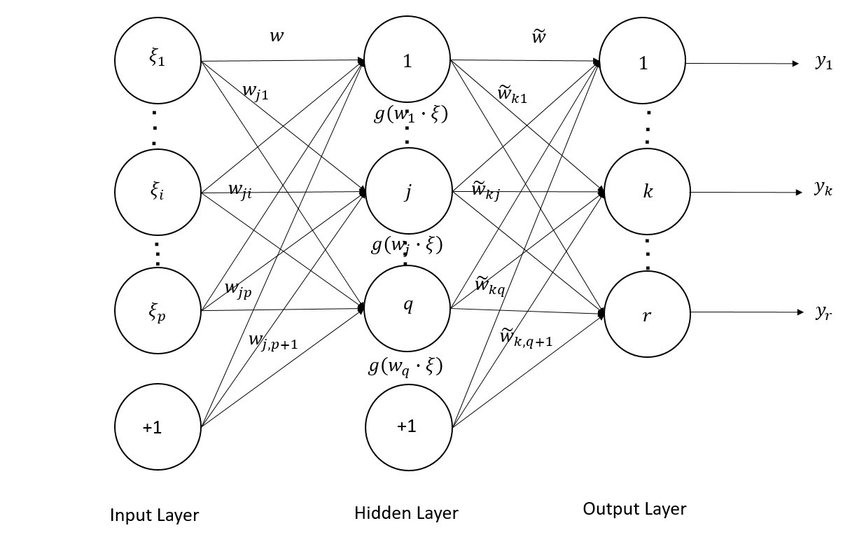
\includegraphics[width=1.0\linewidth, height=4.8cm]{images/ff-neural.png}
            \caption{Kiến trúc mạng Nơ-ron}
            \label{fig:problem:neural-architect}
        \end{figure}
		\end{columns}
	\end{frame}
	\begin{frame}{Huấn luyện mạng Nơ-ron}
	    \begin{itemize}
	    \begin{block}{Phương pháp huấn luyện}
        		    Có 2 lớp phương pháp chính
		    \begin{enumerate}
		        \setlength\itemsep{0.01em}
		        \item Lớp thuật toán sử dụng phương pháp \textbf{gradient-based}.
		        \item Lớp thuật toán \textbf{tiến hóa - NeuroEvolution}.
		    \end{enumerate}
		\end{block}
		\end{itemize}
        \begin{columns}
            \column{.6\linewidth}
    		\begin{itemize}
        		\begin{block}{Phương pháp Gradient}
        		    \begin{itemize}
        		    \item Cho hàm số $f(x), x\in \mathbb{R}$, $x^*$ là tối ưu cục bộ, $x_t$ gần $x^*$, tại đó $f^{'}(x_t) > 0$ thì cách tốt nhất để tìm điểm tối ưu là cập nhật $x_t$ ngược hướng đạo hàm:
        		    \begin{center}
        		        $x_{t+1}=x_t - \eta f^'(x_t)$ với $\eta$ là \textbf{tốc độ học}
        		    \end{center}
        		    \item \textcolor{blue}{Tổng quát với hàm nhiều biến $f(\theta)$}:
        		    \begin{center}
                         $\theta_{t+1} = \theta_t - \eta \bigtriangledown_\theta f(\theta_t)$
                    \end{center}\\
                    \end{itemize}
        		\end{block}
        	\end{itemize}
        	\column{.4\linewidth}
        	    \begin{figure}[ht]
                    \centering
                    \fbox{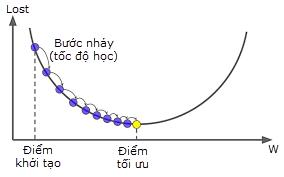
\includegraphics[width=0.7\linewidth]{images/gd.jpg}}
                    \caption{Minh họa cách cập nhật tham số của GD}
                    \label{fig:gd}
                \end{figure}
        \end{columns}
	\end{frame}
	\begin{frame}{Gradient Based và EA}
	    \begin{block}{Gradient Based và EA}
		    Phương pháp dựa trên gradient-based cho đến nay được sử dụng rộng rãi tuy nhiên đang gặp phải một số hạn chế nhất định.
		    \begin{itemize}
		        \setlength\itemsep{0.01em}
		        \item Với những bài toán mà kết quả đầu ra khó xác định, việc tính toán hàm lỗi để cập nhật tham số vô cùng khó khăn.
		        \item Với những mô hình đơn giản nhiều khả năng dẫn tới \emph{cực trị địa phương}.
		    \end{itemize}
		    Vì điều này nhiều nhóm nghiên cứu bắt đầu áp dụng \textbf{EA} để giải quyết các bài toán của mình như \emph{Google Brain, OpenAI, Uber}.  
		\end{block}\pause
		\begin{block}{}
		    \textcolor{red}{Vậy thì huấn luyện mạng Nơ-ron sử dụng EA (NeuroEvolution) hoạt động như thế nào?}
		\end{block}
	\end{frame}
	\begin{frame}{Tiến hóa trong mạng Nơ-ron}
		\begin{itemize}
    		\begin{block}{NeuroEvolution - Khái quát}
    		\begin{itemize}
    		    \setlength\itemsep{0.01em}
    		    \item Được xem xét dưới dạng bài toán tối ưu hộp đen (blackbox optimization)
    		    \item Kiểu gen (genotype) là kiểu cá thể của quần thể sẽ được ánh xạ với các tham số trong mạng Nơ-ron được đánh giá qua hàm \emph{fitness} tương ứng.
    		    \end{itemize}
    		    Vấn đề: \textcolor{red}{Không khai thác được những tri thức đã học được trong các mô hình đã học được trước đó.}
    		\end{block}\pause
    		\begin{block}{Đề xuất: Tiến hóa đa nhiệm trong mạng Nơ-ron}
    		\begin{itemize}
    		    \setlength\itemsep{0.01em}
    		    \item Khai thác mối quan hệ tiềm ẩn của các mạng, tăng tốc độ hội tụ lẫn nhau.
    		    \item Chia thành 2 loại tác vụ tương ứng với các bài toán riêng biệt:
    		    \begin{enumerate}
    		        \setlength\itemsep{0.01em}
    		        \item Mỗi tác vụ tương ứng với một bộ \textbf{\textcolor{red}{dữ liệu, đặc tính dữ liệu}} khác nhau. Ví dụ: bài toán Cart-Pole với môi trường có gravity = 9.8 và gravity = 19.8?
    		        \item Mỗi tác vụ tương ứng với một \textbf{\textcolor{red}{cấu trúc mạng}} khác nhau. Ví dụ: Mô hình mạng với lớp ẩn có 10 nơ-ron và mô hình mạng lớp ẩn 12 nơ-ron.
    		    \end{enumerate}
    		\end{itemize}
    		\textcolor{red}{Trong phạm vi đồ án sẽ giải quyết lần lượt cả 2 bài toán trên}
    		\end{block}
        \end{itemize}
	\end{frame}
	\begin{frame}{Bài toán huấn luyện mạng Nơ-ron}
	    \begin{figure}[ht]
            \centering
            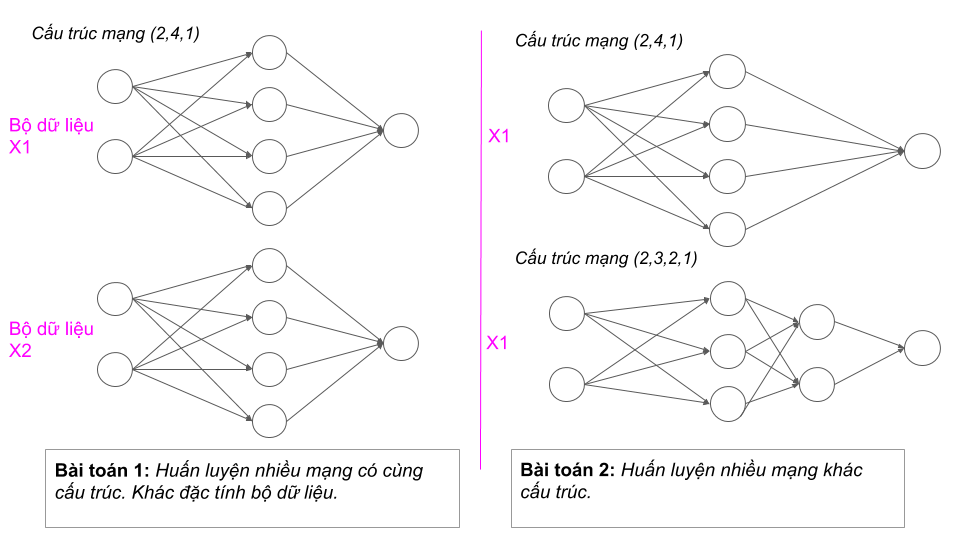
\includegraphics[width=1.0\linewidth]{images/neural-problem.png}
            \caption{Bài toán huấn luyện mạng Nơ-ron}
            \label{fig:problem:neural-problem}
        \end{figure}
	\end{frame}